\chapter{Source Code Layout and Overview}
\label{Source_Code}

OpenVGA is an open-source project, licensed under the GPL. All of the source
code is available on the Internet. The URL is http://openvga.sourceforge.net/
and also contains the snapshot of the project at the point of the completion of
this thesis.

\section{Top-Level}

Also included in the top-level are the standard LICENSE and README text files
which are included within most open-source projects.

\begin{flushleft}

\begin{tabular}{l l}

\textbf{rtl/} & \bigdescript{0.8}{Verilog RTL (Register Transfer Level)
description of the design. There is a Makefile to synthesise the design
using XST and targeting the Spartan-3 FPGA family.} \\
\\

\textbf{sim/} & \bigdescript{0.8}{Verilog RTL (Register Transfer Level)
description files for the test-harnesses of the logic-cores in this
project.}\\
\\

\textbf{src/} & \bigdescript{0.8}{OpenVGA source code for kernel driver, the TTA
assembler, the RISC16 assembler, the cache and text-mode
simulators, and a partial VGABIOS implementation.}	\\
\\

\textbf{tools/} & \bigdescript{0.8}{Scripting files used for tasks such as
assigning data to BRAMs, converting fonts, and a CRT simulator.} \\
\end{tabular}

\end{flushleft}



\section{HDL Hierarchy}

The Verilog source code is consists of both logic-core source files and hardware
testbenches. Simulation test-harness code is in a separate {\texttt sim}
directory.

\begin{flushleft}

\begin{tabular}{l l}
\textbf{rtl/} & \bigdescript{0.75}{The top-level OpenVGA modules, testbenches,
and makefile.}	\\
\\

\textbf{rtl/cpu/} & \bigdescript{0.75}{Both the RISC16 and TTA16 processors, and
hardware testbenches.}	\\
\\

\textbf{rtl/lib/} & \bigdescript{0.75}{Library containing copies of modules not
specific to the OpenVGA project. This includes LFSRs, multiplexors, FIFOs.}	\\
\\

\textbf{rtl/misc/} & \bigdescript{0.75}{Miscellaneous modules, and testbenches,
that are too OpenVGA specific for the ``lib'' directory.}	\\
\\

\textbf{rtl/pci/} & \bigdescript{0.75}{The files for the
PCI-to-Wishbone Bridge logic core and a hardware testbench.}	\\
\\

\textbf{rtl/sdram/} & \bigdescript{0.75}{SDRAM controller logic core modules and
hardware testbench.}	\\
\\

\textbf{rtl/video/} & \bigdescript{0.75}{The OpenVGA video logic core. There are
CRTC, prefetch buffer, redraw logic, and hardware testbench modules.} \\
\end{tabular}

\end{flushleft}



\section{Simulation Test-Harness Hierarchy}

This directory contains the Verilog simulation files for the logic cores within
the \texttt{sim} directory.

\begin{flushleft}

\begin{tabular}{l l}
\textbf{sim/} & \bigdescript{0.75}{The top-level OpenVGA, module
test-harnesses, and Makefile.} \\
\\

\textbf{sim/cpu/} & \bigdescript{0.75}{RISC16 and TTA16 simulation
test-harnesses for use with Verilog simulators.}\\
\\

\textbf{sim/lib/} & \bigdescript{0.75}{Library containing test-harnesses for
modules not specific to the OpenVGA project. This includes test-harnesses for
LFSRs, multiplexers, FIFOs. Additionally, many Xilinx built-in primitives were
emulated and these modules and test-harnesses are within this folder as well.}
\\
\\

\textbf{sim/misc/} & \bigdescript{0.75}{Miscellaneous test-harnesses for
modules that are too OpenVGA specific for the ``lib'' directory.} \\
\\

\textbf{sim/pci/} & \bigdescript{0.75}{Test-harnesses used while developing
the PCI logic core.}	\\
\\

\textbf{sim/sdram/} & \bigdescript{0.75}{SDRAM controller test-harnesses.}	\\
\\

\textbf{sim/video/} & \bigdescript{0.75}{The OpenVGA CRTC, prefetch buffer,
redraw logic, and testbenches.} \\
\end{tabular}

\end{flushleft}


\section{Tools}

There were many scripts and other tools created for this project. They are
typically used for converting data between the many formats used, like font data,
creating Verilog include files, and other post-processing tasks.

Other tools include \texttt{peek}, \texttt{poke}, \texttt{set}, \texttt{test},
and other OpenVGA test applications that were used for developing and testing the
PCI bridge and SDRAM controller. These were run on the host computer that OpenVGA
was attached to.



%============================================================================
\chapter{OpenVGA Components and PCB}
\label{HARDWARE}

This appendix provides more detail of the OpenVGA hardware. The CADSoft
Eagle\texttrademark~schematic, board, and parts-list files are available on the
Internet from http://openvga.sourceforge.net/. OpenVGA uses of a two-layer PCB
for cost and simplicity and the PCB form-factor is a full-height, short, PCI
expansion board with rear I/O panel connectors (see Figure~\ref{HARDWARE__PCB}).
Two-layer PCBs restrict the choice of electronic components due to routing and
signal integrity issues. Data-sheets of high-pinout BGA ICs often recommend
six-layer PCBs or more, for example~\cite{Xilinx_SP3_DS}.

\begin{figure}[h!]
\begin{center}
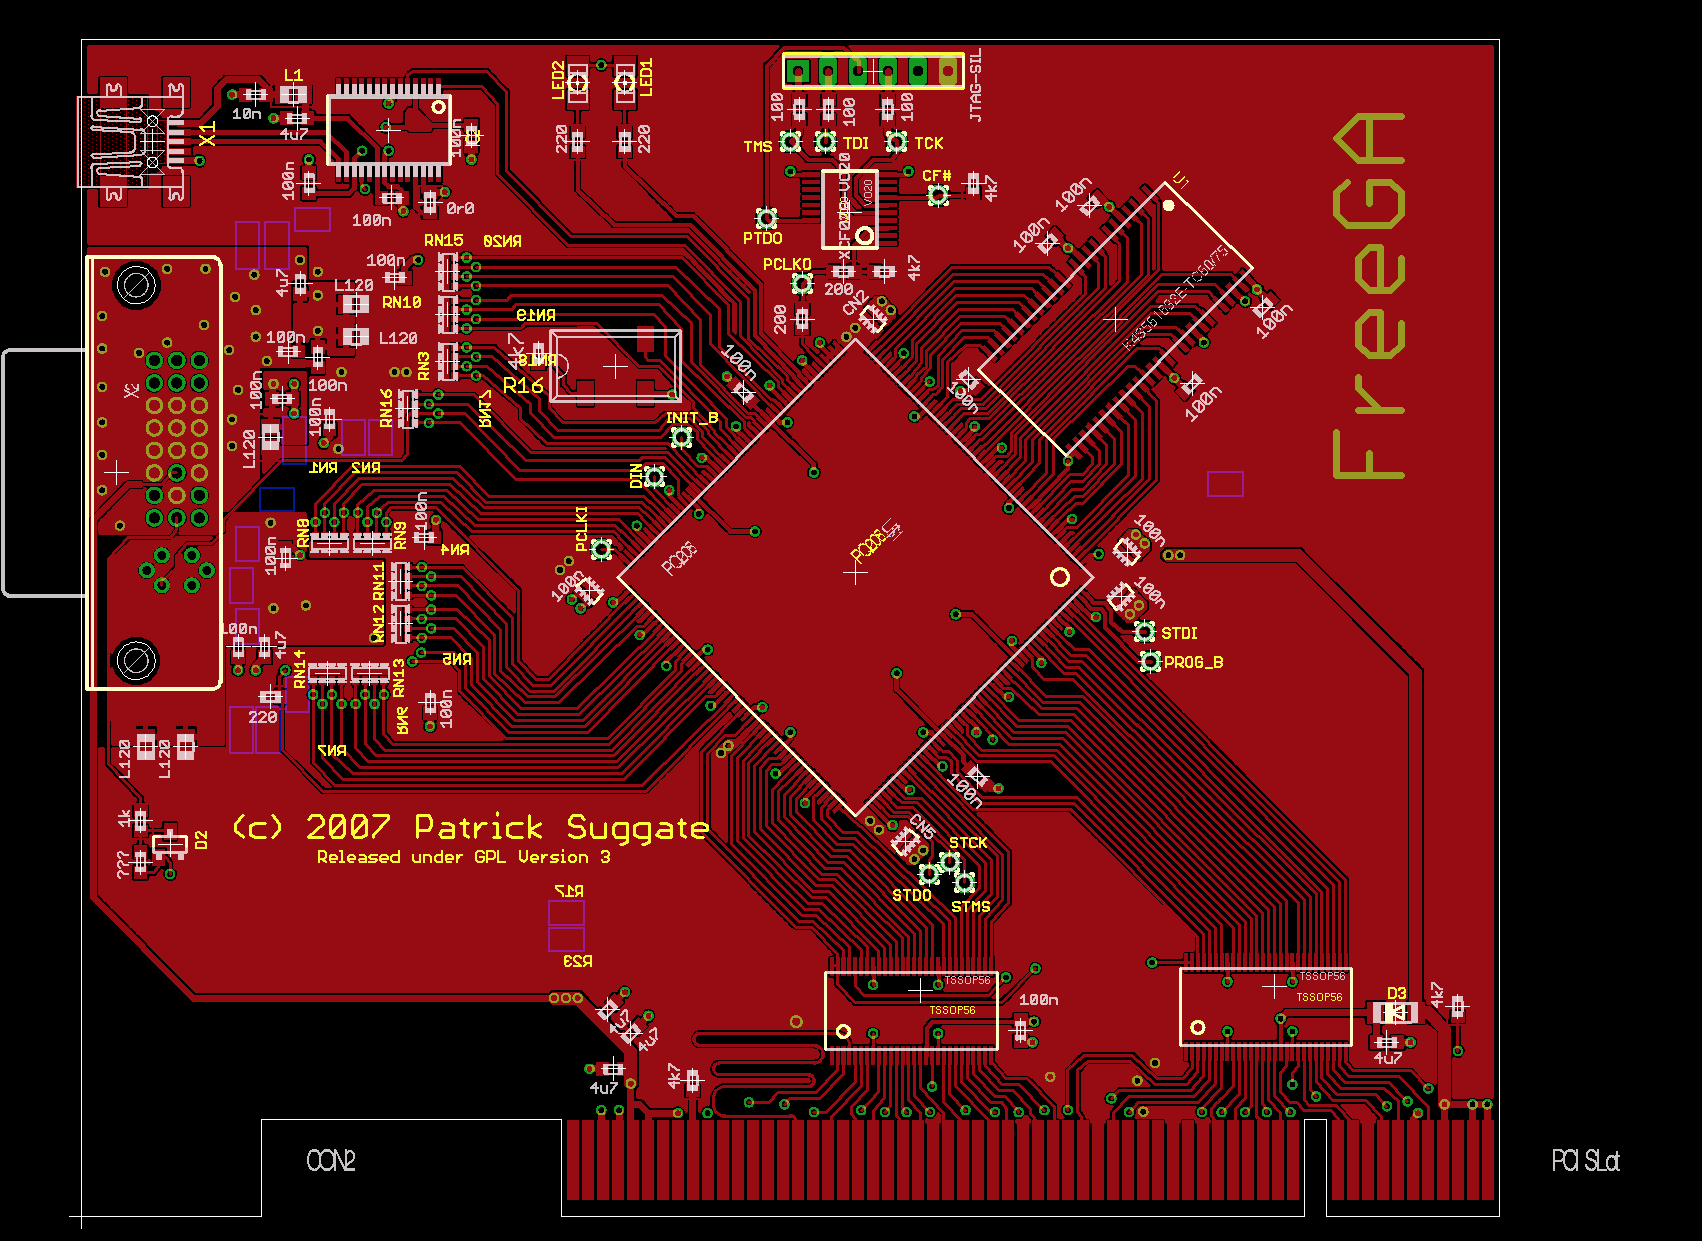
\includegraphics[width=0.49\linewidth]{images/freega3_pcb_art_top.png}
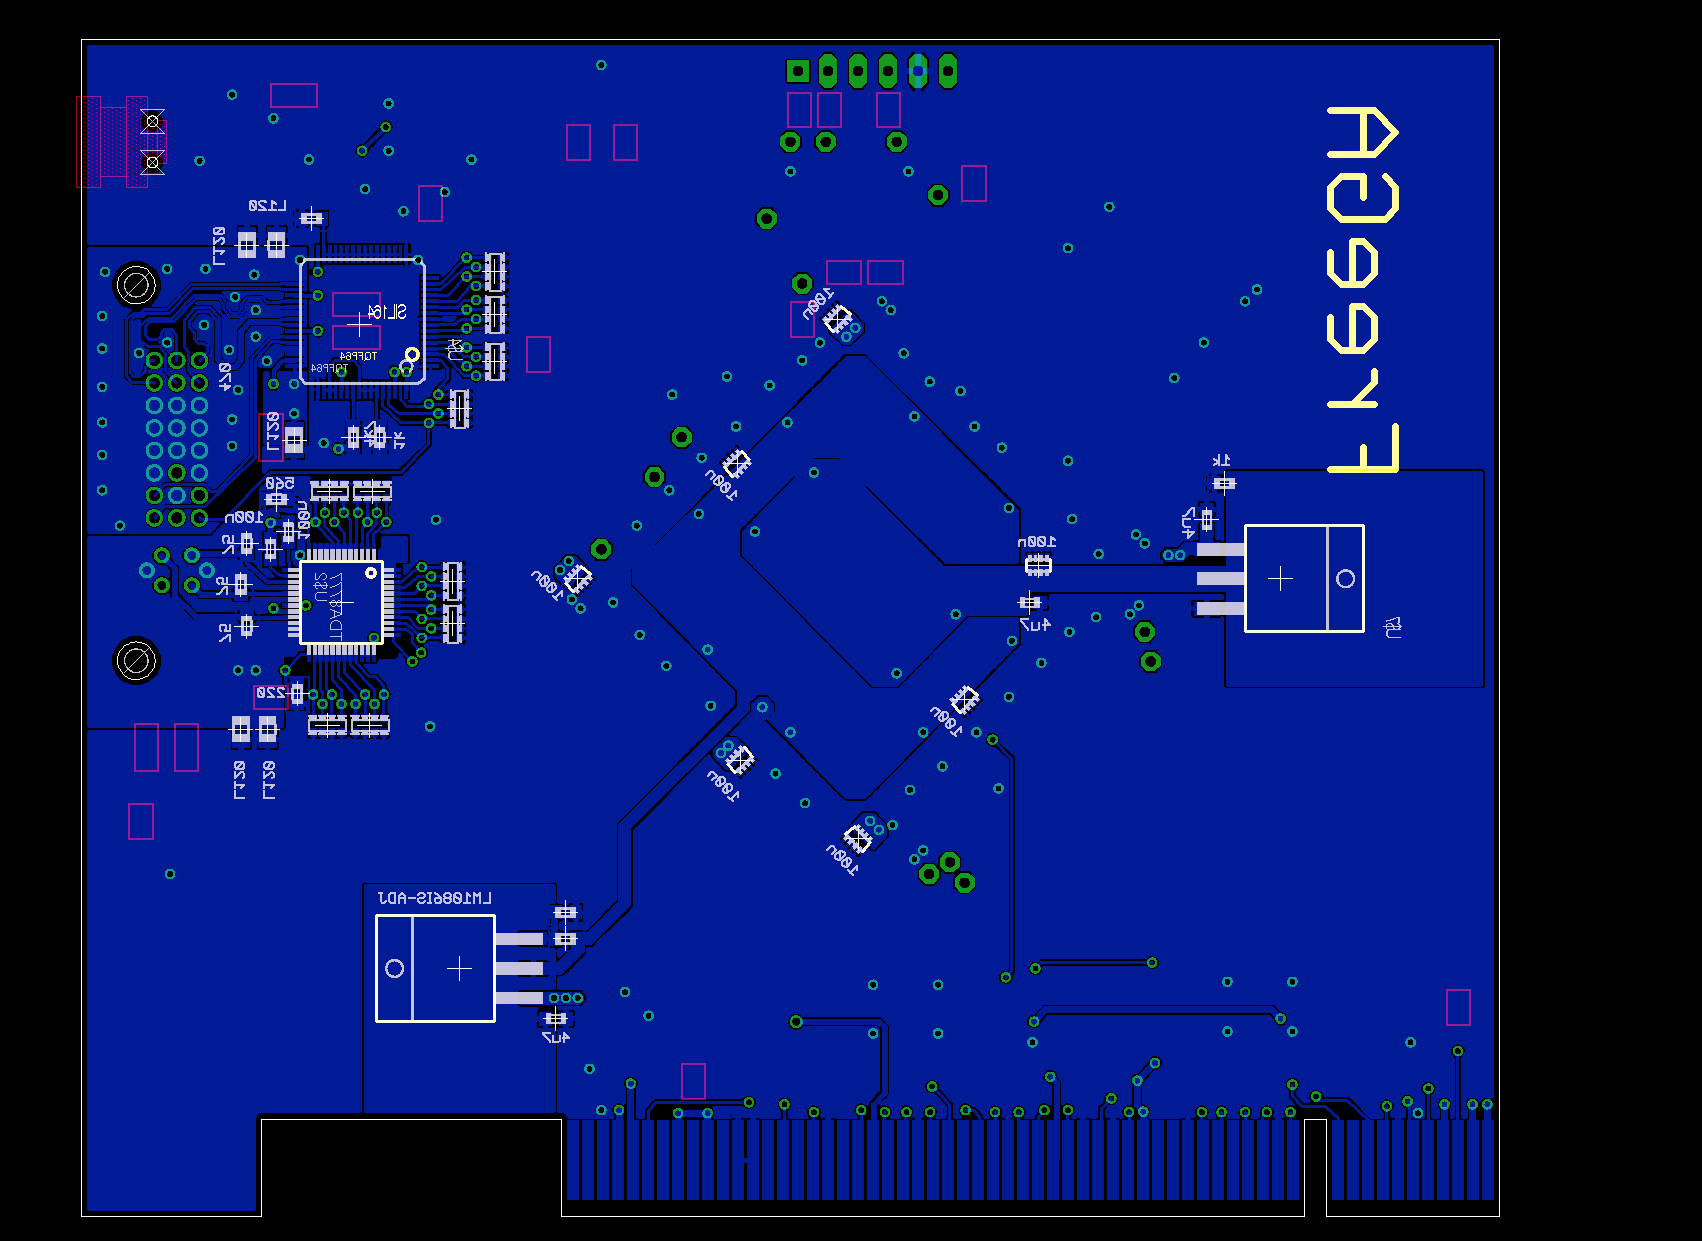
\includegraphics[width=0.49\linewidth]{images/freega3_pcb_art_bot.png}
\end{center}
\caption[OpenVGA PCB artwork, both sides]{OpenVGA PCB artwork, both sides.}
\label{HARDWARE__PCB}
\end{figure}


The FPGA has mostly user assignable inputs and outputs so this allowed flexible
placement of most of the other ICs. The video transmitters could be near the back
edge of the PCB and SDRAM could be placed so as to minimise trace lengths.

The components were laid out with the objective of having the majority of the
signal routing on the top-layer (the component-side) so that the bottom-layer
(the solder-side) could be used for routing the power-supply and ground nets. The
VGA and DVI transmitter ICs were mounted on the solder-side as well, and this was
to simplify routing. The decoupling capacitors and termination resistors were
mounted on both sides of the PCB since they were required to be as close as
possible to their related ICs.


\section{Off-Board Connections}
OpenVGA has connectors for PCI, DVI, VGA (through the DVI connector, using an
adapter), JTAG, and USB (see Figure~\ref{OPENVGA_OpenVGA}. Only the JTAG
connections are connected directly to the FPGA, the rest use encoder or
voltage-translation ICs and are detailed below.


\section{Integrated Circuits}
Table~\ref{HARD_ICs} is a list of the ICs chosen for OpenVGA. More complete
descriptions are included in later sections of this appendix.
Figure~\ref{OPENVGA_OpenVGA} shows the ICs which are on the top (component layer)
of the PCB, the two video encoders, the TMDS encoder and the video DAC are shown
in Figure~\ref{HARD_Bot}.

\begin{table}[h!]
\begin{tabular}{l | l}
Part\#				& Description	\\
\hline
XC3S200-4PQG208C	&	Xilinx Spartan-3 FPGA, 200k Gates	\\
MT48LC4M16A2TG-75	&	Micron 8 MB SDRAM	\\
TDA8777HL/14/C1,15	&	Philips video DAC, 10-bits/colour component	\\
TFP410PAP			&	Texas Instruments TMDS encoder		\\
LM1086IS-ADJ		&	National Semiconductor SMT, adjustable, voltage regulators	\\
CBT16211DDG			&	Fairchild Semiconductor 24 I/O, Bus Switches	\\
XCF04SVOG20C		&	Xilinx 4 Mb, Platform Flash, Serial PROM	\\
FT232RL				&	Future Technology Ddevices International USB UART	\\
SG-8002JA-MPT		&	Epson Toyocom Corporation 50 MHz, SMD oscillator	\\
\end{tabular}
\caption[OpenVGA integrated circuits]{OpenVGA integrated circuits.}
\label{HARD_ICs}
\end{table}


\subsection{The Xilinx Spartan-3 FPGA and SPROM}
The core of OpenVGA is a FPGA which contains the logic necessary for implementing
this display device. The FPGA is a 200 k-Gate, Xilinx Spartan-3, XC3S200 FPGA,
which is from the Xilinx low-cost product range. It has a quantity of
programmable logic that Xilinx considers as approximately equivalent to an IC
with about 200,000 gates.

The FPGA can be programmed using a \gls{jtag} boundary-scan chain or on power-on using a Xilinx SPROM. The
state of the Spartan-3 is lost on power-off~\cite{Xilinx_SP3_DS} so a SPROM
(Serial Programmable Read-Only Memory) is used to restore the state at power-on.
The SPROM is programmed using the JTAG boundary-scan chain as well.

The Spartan-3 requires multiple supply voltages. This Spartan-3 core logic runs
at 1.2 V, the I/O banks at 3.3 V, and the FPGA configuration circuitry at 2.5 V.
This complicates the power-supply routing when using a two-layer PCB, but
decoupling capacitors were used in accordance to Xilinx specifications and no
problems were experienced, even though Xilinx recommends separate power-planes
for each supply.


\subsection{The DVI and VGA Video Encoders}
The DVI TMDS encoder and the VGA video DAC are used to convert the parallel,
digital video signals generated by the FPGA into the signals (analogue for VGA,
TMDS for DVI) used by an attached DVI or VGA computer monitor. The TMDS encoder
and video DAC operate at high frequencies for a two-layer board so termination
resistors are used to improve signal quality. An early development version of
OpenVGA (as shown in Figure~\ref{OPENVGA_Version2}) had significant signal
integrity issues. Neither the DDR SDRAM or the TMDS encoder operated correctly.
The signal waveforms, as displayed on an oscilloscope, had significant undershoot
and overshoot. The current OpenVGA board with the terminating resistors has very
good signal integrity for a two-layer board.

\begin{figure}[h!]
\begin{center}
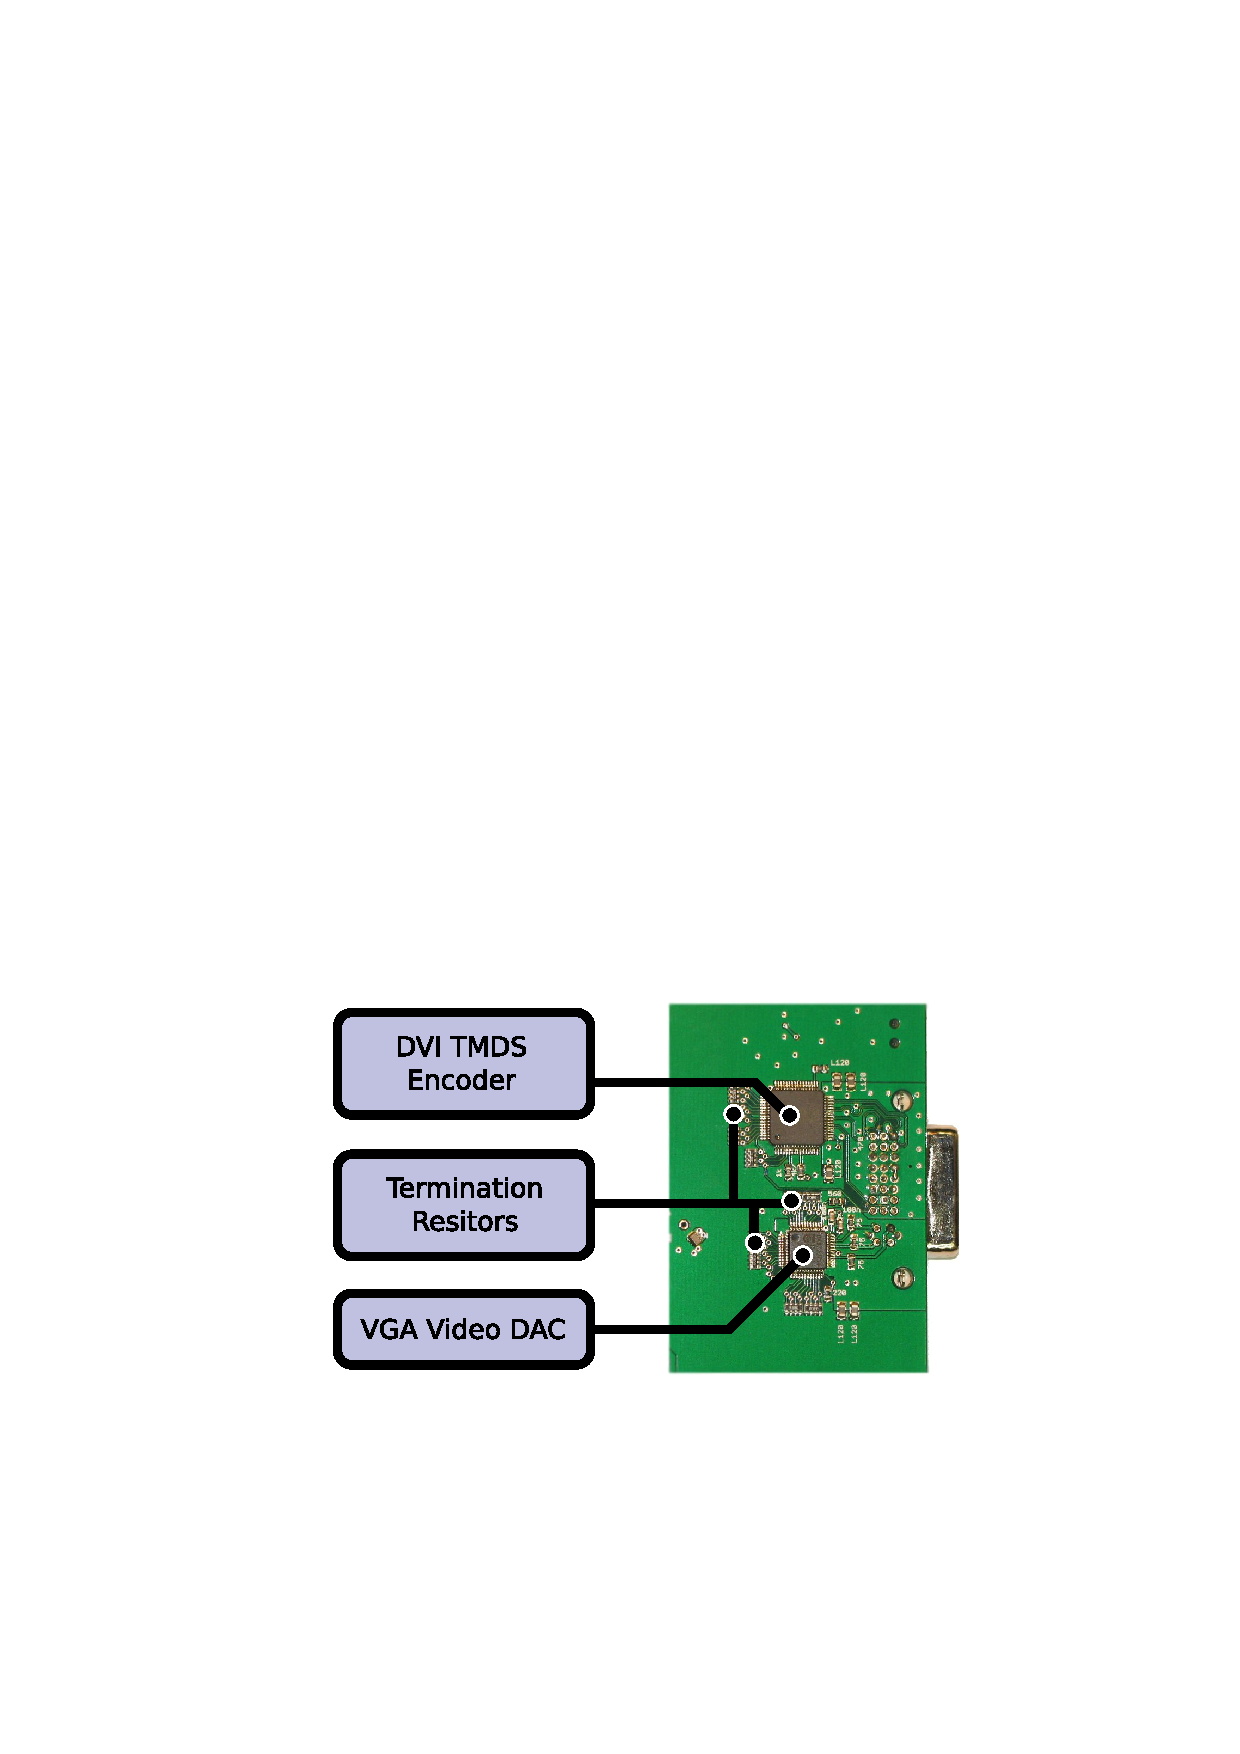
\includegraphics[width=0.5\linewidth]{images/openvga_bot.pdf}
\end{center}
\caption[OpenVGA solder-side components]{OpenVGA solder-side components.}
\label{HARD_Bot}
\end{figure}


\subsection{USB UART}
A logic core was developed which allows the OpenVGA processor to read to, and
write from, the USB UART. This can be used for debugging as well as interfacing
with the many devices which use this standard.


\subsection{PCI Bus Switches}
The PCI Local Bus uses half-wave reflection signalling~\cite{PCI_Spec, PCI_Book}
which causes voltage transients that exceed the maximum operating conditions
specified for the Spartan III family\cite{Xilinx_SP3_DS}. Two 24 pin bus switches
were used to prevent PCI signals from exceeding 3.4 V and -0.7 V. These switches
add a propagation delay of 250 ps~\cite{Bus_Switch_DS}.

